\documentclass[11pt]{report}
\usepackage[pdftex]{graphicx}
\usepackage{henrian-more}
\usepackage{subfig}
 
\makeLayout{Machine Learning: Homework 2}

\begin{document}

\begin{itemize}
  \item \textbf{Email}: chrisbrown@utexas.edu
  \item \textbf{EID}: chb595
\end{itemize}

\section{Algorithm}

The PCA (Principal Component Analysis) algorithm is pretty straightforward, and the MATLAB implementation closely follows the general instructions. The \texttt{hw2FindEigendigits} function is a short 12 lines of code, and could be much shorter by embedding many of the functions. One complication (due to the original version of the assignment) was that sometimes the width of the matrix did not exceed the number of original dimensions of the data (784 in our case), and since the function was required to return a matrix the same size as the input image data, I found that padding it out with zeros was a suitable solution. In those cases where the number of training images was less than 748, truncating the eigenvector matrix to match that number was easy enough. Also, the assignment noted that the eigenvector matrix would need to be sorted by eigenvalues, but MATLAB's \texttt{eig} does that automatically, and only a reverse is needed. However, in line with the assignment, I still sort the eigenvalues and return the corresponding eigenvectors.

\begin{figure}[h]
  \centering
  \subfloat[Using all training data]{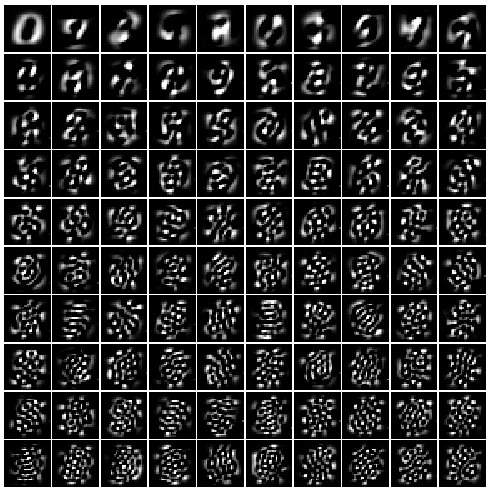
\includegraphics[width=0.4\textwidth]{../plots/100eigenvectors.pdf}}                
  \subfloat[Using 100 training images]{\includegraphics[width=0.4\textwidth]{../plots/100eigenvectors-short.pdf}}
  \caption{The first 100 eigenvectors (ordered in rows, not columns)}
  \label{fig:100eigenvectors}
\end{figure}

\section{Evaluation}

I tried out four basic evaluation metrics:

\begin{itemize}
  \item kNN (k = 1) \hfill (kNN: k-Nearest Neighbors)
  \item kNN (k = 10) -- majority vote
  \item kNN (k = 10) -- weighted vote
  \item Cosine similarity
\end{itemize}

Most of the computation time is spent evaluating each point relative to the training data. It's easy to project all the training/labeled data and the test data into the space of reduced dimensionality quickly, so I only had to do that once per choice of evaluation metric, number of training images, and number of top eigenvectors. But to evaluate a large group of test data, the algorithm would evaluate each one in term, analyzing the entirety of the training data to find the closest points.
If speed was an issue, we could probably do some preprocessing on the training data to assign different regions of the PCA space certain labels, and then the test points could be queried against these regions, instead of all 60,000 training points.

At first, I used kNN with k = 10 and took the most popular label from the resulting list. This ended up being slightly better than kNN with k = 1, since in some cases you can have a particularly sloppy `4' that looks a \emph{lot} like some other specific and also very sloppy `9,' but in general looks more like a `4' than a `9,' based on several other digits. That is, it takes out some of the anomalies. The advantages of this diminshes as we gain more training images, as the PCA space becomes more saturated with examples. But then I realized that this was naive, and that since the \texttt{knnsearch} function returns distances as well as a simple indexation, I could average the distance to all the `4' matches in the top 10, and all the `9' matches, for example, and take the shortest of those. This turned out not to really make a difference, but since it seemed to make more sense, I proceeded to use this metric (weighted kNN, k = 10) for the final analysis.

Cosine similarity (using \texttt{pdist2}, not the cosine option of \texttt{knnsearch}), gave me decent results, but it wasn't nearly as fast or successful as \texttt{knnsearch} using euclidean distances. Also, MATLAB warned me that my data did not seem entirely suitable for the cosine similarity metric, which is probably true.

\begin{figure}[h]
  \centering
  \subfloat[1-NN]{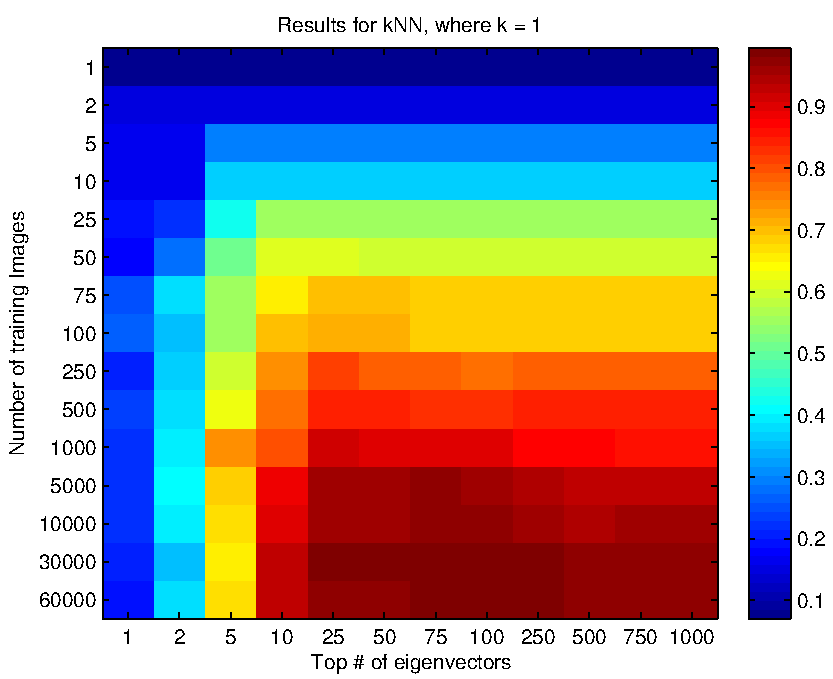
\includegraphics[width=0.22\textwidth]{../plots/metrics-1nn.pdf}}                
  \subfloat[10-NN majority vote]{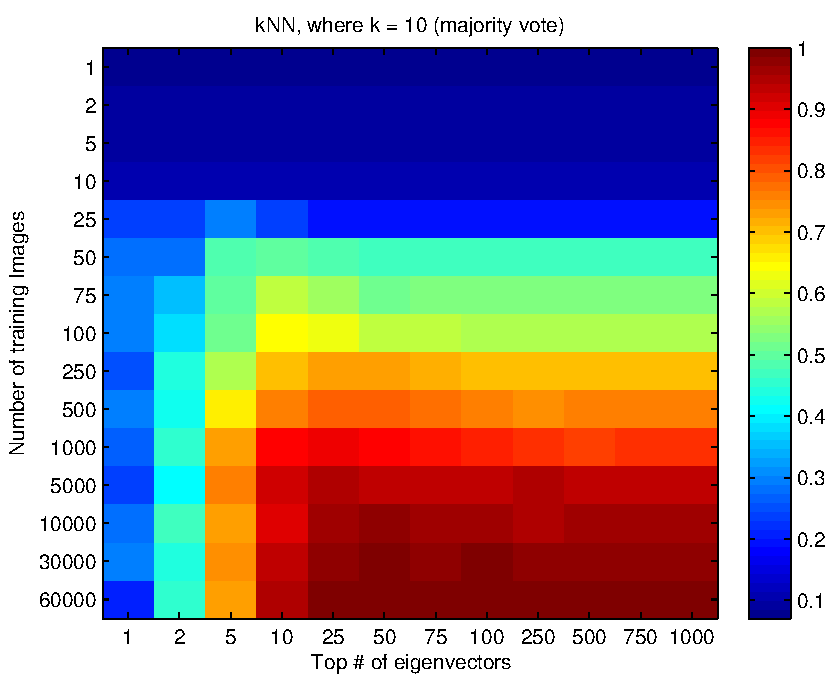
\includegraphics[width=0.22\textwidth]{../plots/metrics-10nn-vote.pdf}}
  \subfloat[10-NN weighted]{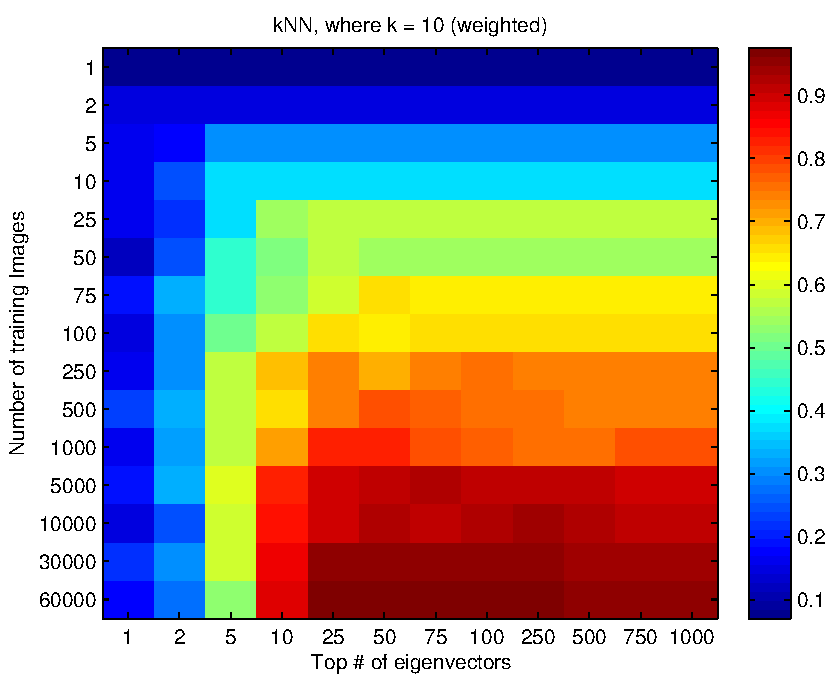
\includegraphics[width=0.22\textwidth]{../plots/metrics-10nn-weighted.pdf}}
  \subfloat[Cosine similarity]{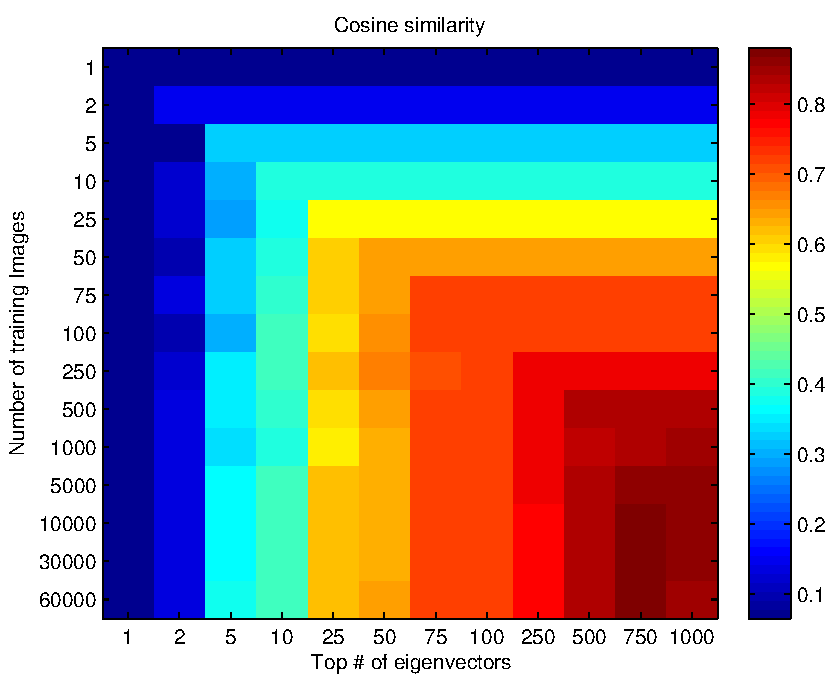
\includegraphics[width=0.22\textwidth]{../plots/metrics-cosine.pdf}}
  \caption{Evaluation metrics}
  \label{fig:metrics}
\end{figure}

\section{Results}


There are two variables we can plot accuracy on: the number of top eigenvectors (the dimensionality of the eigenspace), and the number of training images. I do this for different portions of the test data:

\begin{figure}[h]
  \centering
  \subfloat[Easy 5,000]{\includegraphics[width=0.45\textwidth]{../plots/easy-5000.pdf}}                
  \subfloat[Hard 5,000]{\includegraphics[width=0.45\textwidth]{../plots/hard-5000.pdf}}
  \subfloat[All 10,000]{\includegraphics[width=0.90\textwidth]{../plots/all-10000.pdf}}
  \caption{Results}
  \label{fig:results}
\end{figure}

We see that we can get pretty good results for as few as 500 training images while using just the top 50 eigenvectors. Perhaps the most interesting thing about these graphs is that for fewer training images, in the 100-10,000 range, it helps to truncate the eigenvectors, `de-noising' the data when transforming it into the PCA space, in a way. However, this advantage falls off as we simply use more and more training images (which is just another way of reducing noise in the training dataset).

\end{document}


What happens if you trim the vector down and only use the top n eigenvectors? How accurately can you classify using nearest neighbor using cosine similarity? Plot figures showing the accuracy as the number of training points increases, and as the number of eigenvectors increases.

Must the images be centered exactly? what if they aren't?

What happens if you trim the vector down and only use the top n eigenvectors? How accurately can you classify using the method on page 21 of the lecture notes using the Euclidean distance metric? Plot figures showing the accuracy as the number of training points increases, and as the number of eigenvectors increases.

Write, review, and submit a brief report detailing what you did, how well it worked, and something interesting that you learned. At the beginning of your report include your email address and EID in addition to your name. Also submit your code. Submit using turnin to hychyc07. This is hw2.

